\documentclass[]{elsarticle} %review=doublespace preprint=single 5p=2 column
%%% Begin My package additions %%%%%%%%%%%%%%%%%%%
\usepackage[hyphens]{url}

  \journal{Transport Findings} % Sets Journal name


\usepackage{lineno} % add
\providecommand{\tightlist}{%
  \setlength{\itemsep}{0pt}\setlength{\parskip}{0pt}}

\usepackage{graphicx}
\usepackage{booktabs} % book-quality tables
%%%%%%%%%%%%%%%% end my additions to header

\usepackage[T1]{fontenc}
\usepackage{lmodern}
\usepackage{amssymb,amsmath}
\usepackage{ifxetex,ifluatex}
\usepackage{fixltx2e} % provides \textsubscript
% use upquote if available, for straight quotes in verbatim environments
\IfFileExists{upquote.sty}{\usepackage{upquote}}{}
\ifnum 0\ifxetex 1\fi\ifluatex 1\fi=0 % if pdftex
  \usepackage[utf8]{inputenc}
\else % if luatex or xelatex
  \usepackage{fontspec}
  \ifxetex
    \usepackage{xltxtra,xunicode}
  \fi
  \defaultfontfeatures{Mapping=tex-text,Scale=MatchLowercase}
  \newcommand{\euro}{€}
\fi
% use microtype if available
\IfFileExists{microtype.sty}{\usepackage{microtype}}{}
\bibliographystyle{elsarticle-harv}
\ifxetex
  \usepackage[setpagesize=false, % page size defined by xetex
              unicode=false, % unicode breaks when used with xetex
              xetex]{hyperref}
\else
  \usepackage[unicode=true]{hyperref}
\fi
\hypersetup{breaklinks=true,
            bookmarks=true,
            pdfauthor={},
            pdftitle={An examination of the accessibility implications of a pilot COVID-19 vaccination program in Hamilton, Ontario},
            colorlinks=false,
            urlcolor=blue,
            linkcolor=magenta,
            pdfborder={0 0 0}}
\urlstyle{same}  % don't use monospace font for urls

\setcounter{secnumdepth}{0}
% Pandoc toggle for numbering sections (defaults to be off)
\setcounter{secnumdepth}{0}

% Pandoc citation processing

% Pandoc header
\usepackage{float} \usepackage{xcolor} \floatplacement{figure}{H} \usepackage[margin=1.25in]{geometry}
\usepackage{booktabs}
\usepackage{longtable}
\usepackage{array}
\usepackage{multirow}
\usepackage{wrapfig}
\usepackage{float}
\usepackage{colortbl}
\usepackage{pdflscape}
\usepackage{tabu}
\usepackage{threeparttable}
\usepackage{threeparttablex}
\usepackage[normalem]{ulem}
\usepackage{makecell}
\usepackage{xcolor}



\begin{document}
\begin{frontmatter}

  \title{An examination of the accessibility implications of a pilot COVID-19
vaccination program in Hamilton, Ontario}
    \author[McMaster University]{Antonio Paez\corref{1}}
   \ead{paezha@mcmaster.ca} 
    \author[University of Toronto Scarborough]{Christopher D. Higgins}
   \ead{cd.higgins@utoronto.ca} 
      \address[McMaster University]{School of Earth, Environment and Society, McMaster University, Hamilton,
ON, L8S 4K1, Canada}
    \address[University of Toronto Scarborough]{Department of Geography \& Planning, University of Toronto Scarborough,
1265 Military Trail, Toronto, ON M1C1A4}
      \cortext[1]{Corresponding Author}
  
  \begin{abstract}
  The province of Ontario in Canada announced the pilot for a new
  vaccination program, with designated pharmacies across the province now
  able to offer COVID-19 vaccines. The accessibility of this program
  raises questions about the cost of travel and the distribution of the
  cost among the population. In our examination of the City of Hamilton we
  find that selected sites do not serve well the rural and urban
  population of Hamilton, and that the associated cost of travel is
  expected to be disproportionally borne by lower income populations.
  Modest additions to the list of pilot sites in the city can
  substantially alleviate this inequity.
  \end{abstract}
  
 \end{frontmatter}

\hypertarget{research-questions-and-hypotheses}{%
\section{Research Questions and
Hypotheses}\label{research-questions-and-hypotheses}}

Along with the provision of health care facilities to treat severe cases
of COVID-19 (Pereira, C. K. V. S. Braga, et al., 2021), another front in
the fight against the pandemic is the rolling out of vaccination
programs. The Province of Ontario, in Canada, announced on April 1st
2021 the expansion of a pilot program to offer vaccines in pharmacies in
the City of
Hamilton\footnote{\url{https://www.cbc.ca/news/canada/hamilton/astrazeneca-vaccine-hamilton-1.5972704}}.
This program is in addition to dedicated vaccination centers for people
aged 70+. Twenty pharmacies in Hamilton were added to an earlier list of
325 locations in other cities across the province, and the program was
extended to people aged 55 years old and over.

Critics were swift to point out that the list of pharmacies approved for
Hamilton by the province were mostly located in lower density parts of
the city that are not well serviced by transit and are difficult to
reach by
foot\footnote{See inter alia: \url{https://twitter.com/RyanMcGreal/status/1378027149790224386?s=20} and \url{https://twitter.com/NrinderWard3/status/1378679195514060801?s=20}.}.
Indeed, as seen in Figure \ref{fig:pharmacies-and-regions}, a vast
majority of the pharmacies are in suburban Hamilton. The issue is
somewhat less clear-cut when we consider that Hamilton's population
skews suburban (see Figure \ref{fig:population-map}). Given the target
demographic for the program, it is possible that suburban sites could be
convenient for mature adults and young old: the population aged 55 to 69
in Hamilton is approximately 58,710 suburban, 35,490 urban, and only
8,360 rural. Nevertheless, the selection of sites by the province raises
some important
questions\footnote{The decision-making process to select these sites appears to have been opaque, and the typically inert Major of the city was caught flat footed by the announcement; see: \url{https://twitter.com/FredEisenberger/status/1378350123114242053?s=20}}.
As Yu et al. (2021) note, good geographical coverage is a key element
for a successful vaccination campaign; at the same time, siting
vaccinations sites in car-oriented locations may introduce inequities in
access.

In this research, we investigate the accessibility implications of the
sites selected for the pilot vaccination program. Concretely, we ask:

\begin{itemize}
\tightlist
\item
  What is the estimated cost of travel to reach the vaccination sites,
  assuming that every person requires a vaccine?
\item
  What is the distribution of this cost across the population of the
  city?
\item
  How does the cost and its distribution change with the addition of
  candidate sites in urban Hamilton?
\end{itemize}

We concentrate on the 55 to 69 years old population segment because the
older 70+ group have access to other dedicated facilities besides those
in the provincial pilot.

\begin{figure}

{\centering 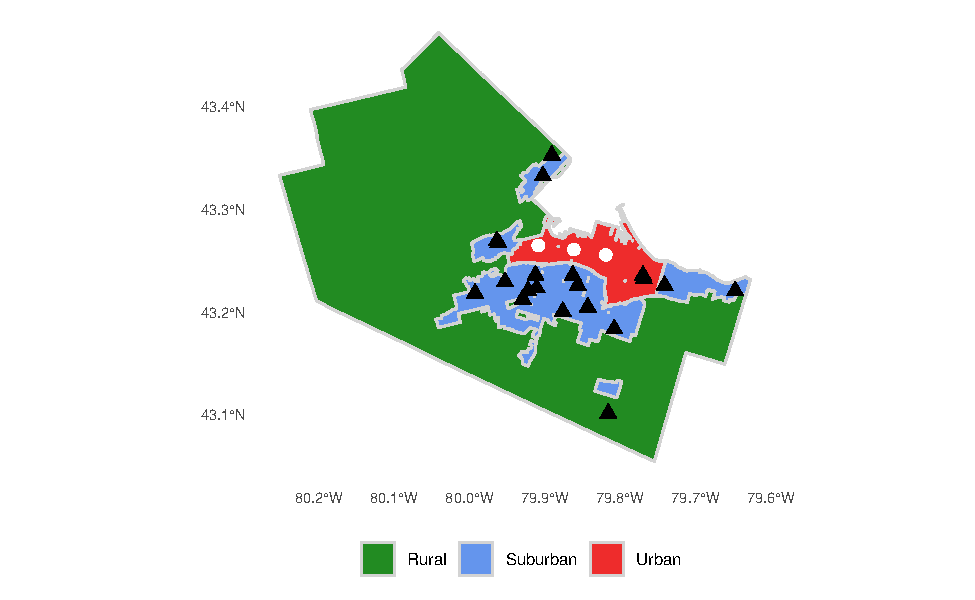
\includegraphics{Accessibility-Vaccination-Sites-Hamilton_files/figure-latex/pharmacies-map-1} 

}

\caption{\label{fig:pharmacies-and-regions}Regions with the City of Hamilton; the location of pharmacies in pilot is shown (black triangles) and urban locations for scenario analysis (white circles)}\label{fig:pharmacies-map}
\end{figure}

\begin{figure}

{\centering 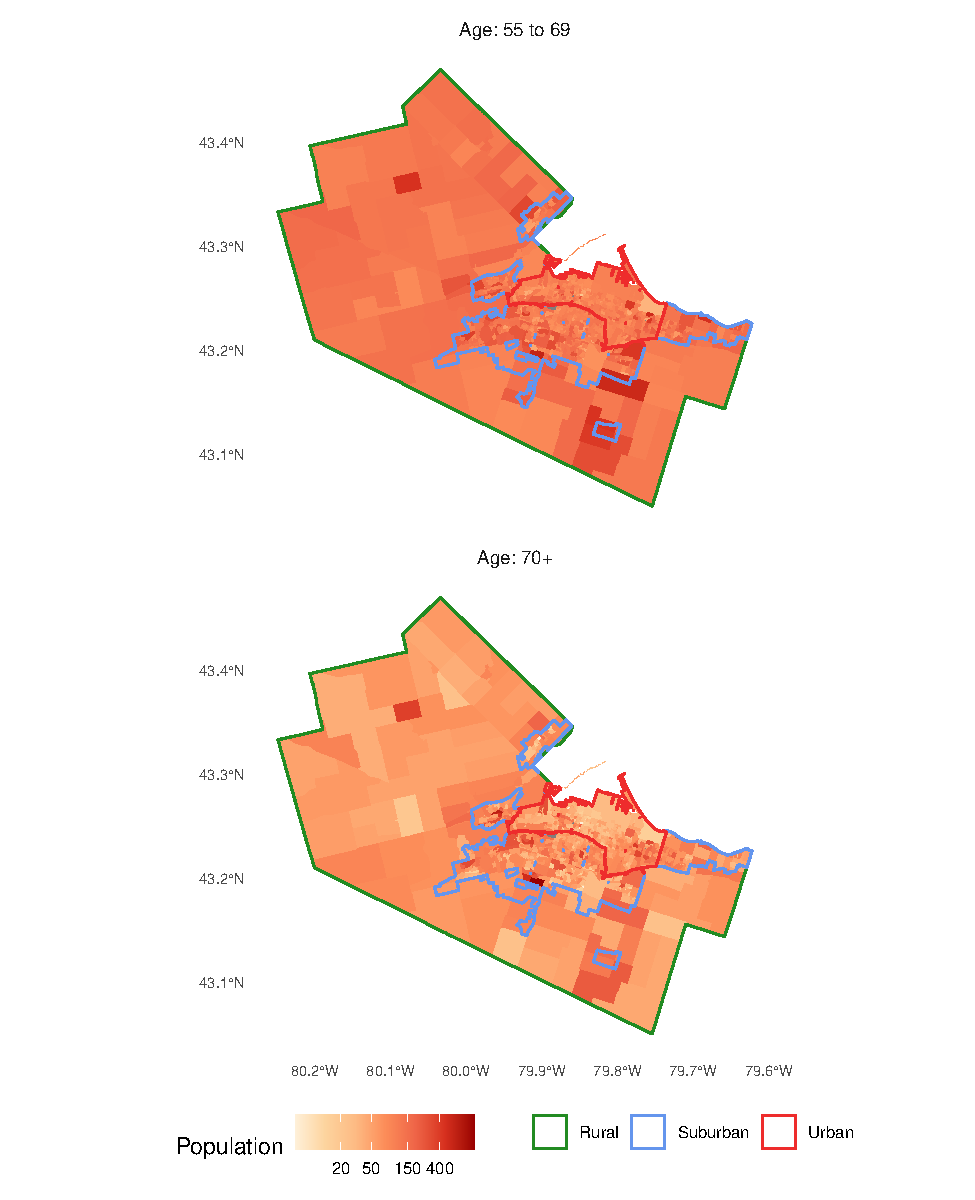
\includegraphics{Accessibility-Vaccination-Sites-Hamilton_files/figure-latex/population-map-1} 

}

\caption{\label{fig:population-map}Distribution of population age 55+ in the City of Hamilton}\label{fig:population-map}
\end{figure}

\hypertarget{methods-and-data}{%
\section{Methods and Data}\label{methods-and-data}}

\hypertarget{data}{%
\section{Data}\label{data}}

We use data from the following sources.

\hypertarget{open-hamilton}{%
\subsubsection{Open Hamilton}\label{open-hamilton}}

From the open data portal of the City of
Hamilton\footnote{\url{https://open.hamilton.ca/}} we obtained
boundaries for the city's various regions (the definition of urban,
suburban, and rural regions follows the classification of development
applications).

\hypertarget{statistics-canada}{%
\subsubsection{Statistics Canada}\label{statistics-canada}}

Population and income statistics at the level of Dissemination Areas
(DAs) were retrieved using the package \texttt{cancensus} (von Bergmann
et al., 2021). Dissemination Areas are the smallest publicly available
census geography in Canada. We use data from the 2016 Population Census.

\hypertarget{transportation-tomorrow-survey}{%
\subsubsection{Transportation Tomorrow
Survey}\label{transportation-tomorrow-survey}}

Data about modal split by age by place of residence were downloaded from
the Data Retrieval System of the Transportation Tomorrow Survey
(TTS)\footnote{\url{http://dmg.utoronto.ca/}}. The data are geocoded at
the level of Traffic Analysis Zones (TAZ).

\hypertarget{other}{%
\subsubsection{Other}\label{other}}

The locations of pharmacies in the pilot were obtained from public
records and geocoded. Three urban sites not in the program were also
identified and geocoded for comparison purposes. In addition, we
converted all recorded residential parcels in the City of Hamilton to
points on the road network. Each point includes information about the
number of residential units in the parcel.

\hypertarget{methods}{%
\section{Methods}\label{methods}}

We used the population aged 55 to 59 y.o. in each Dissemination Area to
calculate the average number of people per dwelling. This value was then
assigned proportionally to the number of dwellings per parcel. The
median total household income of the corresponding DAs was joined to the
parcels. In addition, we calculated the proportion of trips by mode from
the total number of trips by each of the three modes retrieved from the
TTS data. These proportions were joined to the parcel data based on
their corresponding TAZ. The package \texttt{r5r} (Pereira, Saraiva, et
al., 2021) was used to calculate the travel time from each parcel to all
pharmacies by three modes: car, transit, and walking. For routing
purposes we used a cutoff value of 180 min and a maximum walking
distance of 10,000 m.

Once we obtained travel time tables with population, proportion of trips
by mode, and income information, we calculated the expected travel time
\(ett\) from each parcel \(i\) to a pharmacy \(j\) as follows: \[
ett_i = p^c_i \min(tt^c_{ij}) + p^t_i \min(tt^t_{ij}) + p^w_i \min(tt^w_{ij})
\] \noindent where \(p^k_i\) is the proportion of trips by mode \(k\) in
the TAZ of parcel \(i\), and \(tt^k_{ij}\) is the vector of travel times
from parcel \(i\) to the pharmacies. In other words, the expected travel
time is the weighted sum of travel times to the nearest pharmacy, with
the weights given by the expected modal split in the TAZ.

The expected travel time \(i\) was multiplied by the population in
parcel \(i\) to obtain a measure of person-hours of travel (\(PHT\)) as
follows: \[
PHT_i = P_i\cdot ett_i
\]

Please note that this paper is a reproducible research document (see
Brunsdon and Comber, 2020) conducted using open source tools for
transportation analysis (Lovelace, 2021). The code and data necessary to
reproduce the analysis are available in a public
repository\footnote{\url{https://github.com/paezha/Accessibility-Pharmacies-Hamilton-Vaccines}}.

\hypertarget{findings}{%
\section{Findings}\label{findings}}

The top panel of Figure \ref{fig:maps-baseline} shows the average
expected travel time by TAZ in Hamilton. It is apparent that travel
times tend to be lower in much of suburban Hamilton, and higher in the
urban core and some rural parts of the city, particularly to the west.
This is unsurprising, given the higher probability of travel by car and
the predominantly suburban character of the vaccination sites. However,
even accounting for the distribution of population, this leads to large
disparities in the number of person-hours of travel across the city,
with a concentration of the burden of travel in the urban core and the
rural west (see bottom panel of Figure \ref{fig:maps-baseline}).

The disparities are not trivial.

As seen in Table \ref{tab:distribution-results}, under the pilot program
approximately 36.42\% of people live in DAs in the bottom 40\% of the
median household income scale, but they account for 51.98\% of the total
person-hours of travel. In contrast, 44.5\% of people aged 55 to 69 in
DAs in the top 40\% of the median household income scale accrue only
35.03\% of the total person-hours of travel. Where the mean travel time
of residents of DAs with high median household income is 6 minutes,
residents of lower income DAs average 12 minutes in travel time. In
addition to longer average travel time, residents in lower income DAs
also see substantially larger variations in travel times, and some may
face considerably longer travel times (see top-left panel in Figure
\ref{fig:results}).

There are also important disparities by region. As shown in Table
\ref{tab:distribution-results}, the urban and rural populations in
Hamilton are approximately 42.75\% of the population but they bear
69.25\% of the total person-hours of travel, with also much greater
variability in expected travel times (Figure \ref{fig:results},
bottom-left panel).

For comparison purposes we consider a scenario with some modest
additions to the list of pharmacies in the provincial pilot. We repeat
the analysis, but include the three urban sites shown in white circles
in Figure \ref{fig:pharmacies-and-regions}. The results of this scenario
appear in the last two columns of Table \ref{tab:distribution-results}
and the two right panels of Figure \ref{fig:results}. We begin by noting
that all income groups benefit from the addition of these three sites
with shorter mean trip durations; the most remarkable difference is the
large reduction in the disparities between residents in DAs with
different levels of income. The top-right panel of Figure
\ref{fig:results} shows that the distribution of expected travel time is
now more in line for all income groups, even if the bottom two income
quintiles still have somewhat wider spreads. With respect to the
distribution of expected travel time and person-hours of travel by
region, unsurprisingly the addition of three urban vaccination sites in
the scenario makes a difference for urban residents but not for rural
residents.

The results indicate that the locations chosen by the province for the
pilot vaccination program do not serve well urban or rural residents of
the city, and there are some important questions regarding equity of
access to the program, with a disproportionate burden in the cost of
travel falling on lower income urban populations and rural populations.
A scenario did not consider candidate sites in a systematic way.
Nonetheless, selection of three sensible urban locations does much to
alleviate disparities in the burden of transportation. On the other
hand, unlike the urban context where there are numerous candidate
locations that could be chosen for a vaccination program, there are not
many candidate locations in rural regions of the city. Increasing access
in rural Hamilton likely will involve an expansion of existing mobile
vaccination pop-up
clinics\footnote{\url{https://www.hamilton.ca/government-information/news-centre/news-releases/hamiltons-covid-19-vaccination-program-expansion-1}}.

\begin{figure}

{\centering 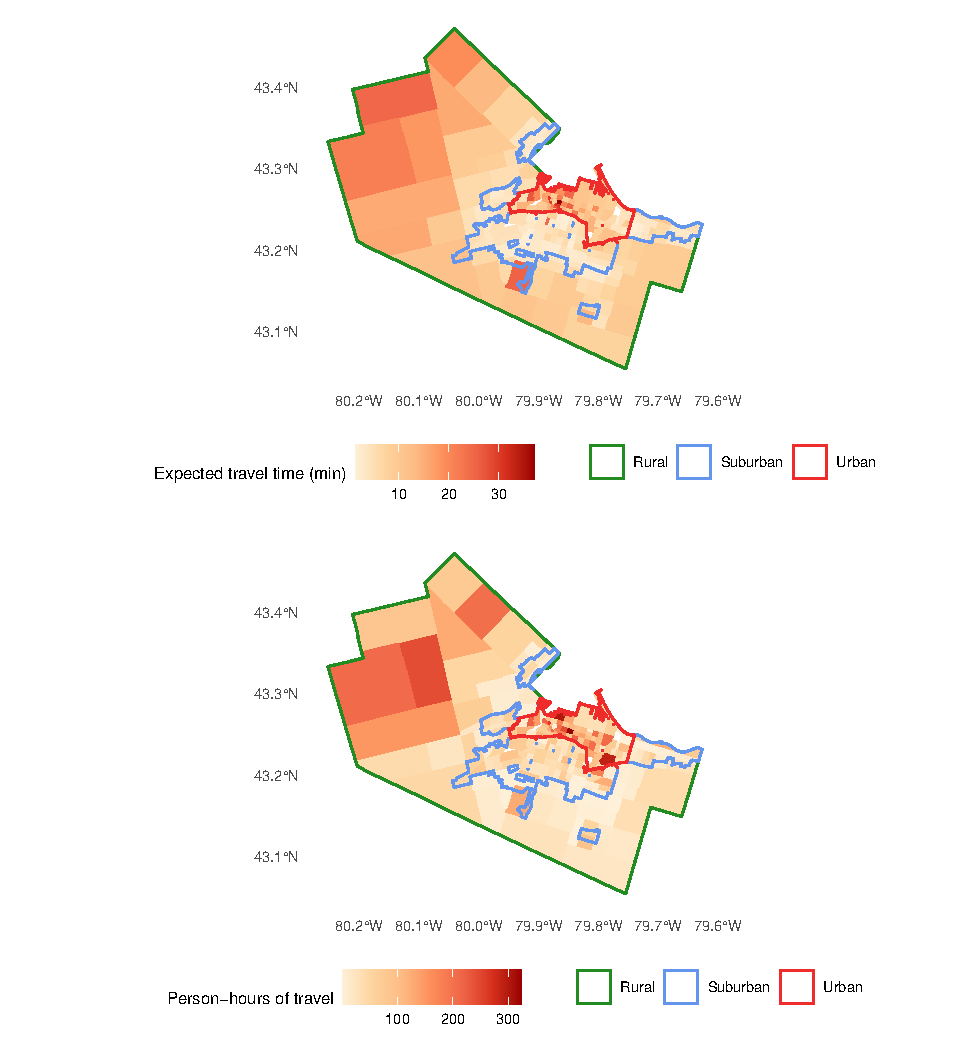
\includegraphics{Accessibility-Vaccination-Sites-Hamilton_files/figure-latex/figure-maps-baseline-1} 

}

\caption{\label{fig:maps-baseline}Average expected travel time by TAZ (in minutes) and total person-hours of travel by TAZ.}\label{fig:figure-maps-baseline}
\end{figure}

\begin{table}

\caption{\label{tab:table-results}\label{tab:distribution-results}Distribution of person-hours of travel (PHT) by median total household income and region: pilot locations only, and scenario with three urban locations added}
\centering
\resizebox{\linewidth}{!}{
\begin{tabular}[t]{lccccc}
\toprule
\multicolumn{2}{c}{ } & \multicolumn{2}{c}{Pilot Program} & \multicolumn{2}{c}{Scenario} \\
\cmidrule(l{3pt}r{3pt}){3-4} \cmidrule(l{3pt}r{3pt}){5-6}
Group & Population & Total PHT & Hours per person & Total PHT & Hours per person\\
\midrule
\addlinespace[0.3em]
\multicolumn{6}{l}{\textbf{Income Quintile}}\\
\hspace{1em}\cellcolor{gray!6}{Top 20\%} & \cellcolor{gray!6}{23297.315} & \cellcolor{gray!6}{2243.857} & \cellcolor{gray!6}{0.096} & \cellcolor{gray!6}{2146.558} & \cellcolor{gray!6}{0.092}\\
\hspace{1em}Second 20\% & 22356.413 & 2471.952 & 0.111 & 2351.858 & 0.105\\
\hspace{1em}\cellcolor{gray!6}{Third 20\%} & \cellcolor{gray!6}{19570.061} & \cellcolor{gray!6}{1749.497} & \cellcolor{gray!6}{0.089} & \cellcolor{gray!6}{1563.978} & \cellcolor{gray!6}{0.080}\\
\hspace{1em}Fourth 20\% & 17729.139 & 2928.959 & 0.165 & 1950.312 & 0.110\\
\hspace{1em}\cellcolor{gray!6}{Bottom 20\%} & \cellcolor{gray!6}{19629.952} & \cellcolor{gray!6}{4068.548} & \cellcolor{gray!6}{0.207} & \cellcolor{gray!6}{2388.422} & \cellcolor{gray!6}{0.122}\\
\addlinespace[0.3em]
\multicolumn{6}{l}{\textbf{Region}}\\
\hspace{1em}Rural & 8356.963 & 1730.268 & 0.207 & 1730.242 & 0.207\\
\hspace{1em}\cellcolor{gray!6}{Suburban} & \cellcolor{gray!6}{58711.629} & \cellcolor{gray!6}{4138.482} & \cellcolor{gray!6}{0.070} & \cellcolor{gray!6}{4138.392} & \cellcolor{gray!6}{0.070}\\
\hspace{1em}Urban & 35491.942 & 7588.590 & 0.214 & 4527.021 & 0.128\\
\bottomrule
\multicolumn{6}{l}{\rule{0pt}{1em}\textit{Note: }}\\
\multicolumn{6}{l}{\rule{0pt}{1em}The population totals differ due to small differences in the classification of the regions}\\
\end{tabular}}
\end{table}

\begin{figure}

{\centering 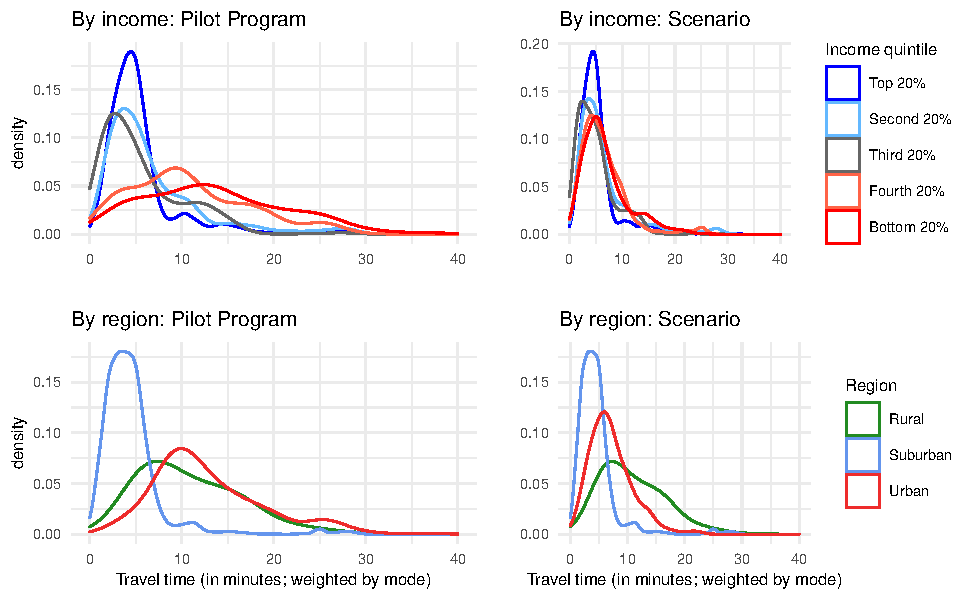
\includegraphics{Accessibility-Vaccination-Sites-Hamilton_files/figure-latex/figure-results-1} 

}

\caption{\label{fig:results}Distribution of expected travel time for different population groups}\label{fig:figure-results}
\end{figure}

\hypertarget{references}{%
\section*{References}\label{references}}
\addcontentsline{toc}{section}{References}

\hypertarget{refs}{}
\leavevmode\hypertarget{ref-Brunsdon2020opening}{}%
Brunsdon, C., Comber, A., 2020. Opening practice: Supporting
reproducibility and critical spatial data science. Journal of
Geographical Systems 1--20.
doi:\href{https://doi.org/10.1007/s10109-020-00334-2}{10.1007/s10109-020-00334-2}

\leavevmode\hypertarget{ref-Lovelace2021open}{}%
Lovelace, R., 2021. Open source tools for geographic analysis in
transport planning. Journal of Geographical Systems.
doi:\href{https://doi.org/10.1007/s10109-020-00342-2}{10.1007/s10109-020-00342-2}

\leavevmode\hypertarget{ref-Pereira2021geographic}{}%
Pereira, R.H.M., Braga, C.K.V.S., Mendes and Serra, L., Amaral, P.B.,
Gouveia, N., Paez, A., 2021. Geographic access to covid-19 healthcare in
brazil using a balanced float catchment area approach. Social Science \&
Medicine 273, 113773.
doi:\href{https://doi.org/https://doi.org/10.1016/j.socscimed.2021.113773}{https://doi.org/10.1016/j.socscimed.2021.113773}

\leavevmode\hypertarget{ref-Pereira2021r5r}{}%
Pereira, R.H.M., Saraiva, M., Herszenhut, D., Braga, C.K.V., Conway,
M.W., 2021. R5r: Rapid realistic routing on multimodal transport
networks with r\textsuperscript{5} in r. Findings.
doi:\href{https://doi.org/10.32866/001c.21262}{10.32866/001c.21262}

\leavevmode\hypertarget{ref-vonBergmann2021cancensus}{}%
von Bergmann, J., Shkolnik, D., Jacobs, A., 2021. Cancensus: R package
to access, retrieve, and work with canadian census data and geography.

\leavevmode\hypertarget{ref-Yu2021sustained}{}%
Yu, J.H., Jeong, H.J., Kim, S.J., Lee, J.Y., Choe, Y.J., Choi, E.H.,
Cho, E.H., 2021. Sustained vaccination coverage during the coronavirus
disease 2019 epidemic in the republic of korea. Vaccines 9, 8.
doi:\href{https://doi.org/10.3390/vaccines9010002}{10.3390/vaccines9010002}


\end{document}


